\documentclass[tikz,border=3pt]{standalone}
\usepackage[utf8]{inputenc}
\usepackage[T1]{fontenc}
\usepackage{lmodern}
\renewcommand{\familydefault}{\sfdefault}
\usepackage{sansmath}\sansmath
\usepackage{pgfplots}\pgfplotsset{compat=1.18,/pgf/number format/use comma,/pgf/number format/1000 sep={.}}
\usetikzlibrary{arrows.meta,calc,positioning,decorations.pathmorphing,patterns}
% paleta del sitio
\definecolor{nar}{HTML}{E8680C}\definecolor{narc}{HTML}{FFB35C}\definecolor{hielo}{HTML}{FFF3E8}
\definecolor{tinta}{HTML}{1D1D1F}\definecolor{gris}{HTML}{6E6E73}\definecolor{lila}{HTML}{7C5CF0}
\definecolor{azul}{HTML}{2F6FD6}\definecolor{menta}{HTML}{17A673}\definecolor{coral}{HTML}{E8342A}
% organelos
\tikzset{
 mito/.pic={
  \draw[nar!75!black,fill=narc!55,line width=0.6pt] (0,0) ellipse (0.5 and 0.24);
  \begin{scope}\clip (0,0) ellipse (0.42 and 0.17);
   \fill[hielo] (-0.5,-0.3) rectangle (0.5,0.3);
   \foreach \x/\s in {-0.3/1,-0.15/-1,0/1,0.15/-1,0.3/1} \draw[nar!75!black,line width=0.7pt] (\x,-0.2*\s) -- (\x,0.07*\s);
  \end{scope}
  \draw[nar!75!black,line width=0.6pt] (0,0) ellipse (0.42 and 0.17);
 },
 cloro/.pic={
  \draw[menta!55!black,fill=menta!30,line width=0.6pt] (0,0) ellipse (0.55 and 0.27);
  \draw[menta!55!black,line width=0.4pt] (0,0) ellipse (0.49 and 0.22);
  \draw[menta!55!black,line width=0.6pt] (-0.36,0)--(0.36,0);
  \foreach \x in {-0.26,0,0.26} \foreach \y in {-0.105,-0.035,0.035,0.105} \fill[menta!55!black] (\x-0.07,\y-0.025) rectangle (\x+0.07,\y+0.025);
 },
 golgi/.pic={
  \foreach \i in {0,1,2,3} {
   \draw[lila!75!black,line width=4.2pt,line cap=round] (0.17*\i,-0.55+0.07*\i) to[bend right=40] (0.17*\i,0.55-0.07*\i);
   \draw[lila!22,line width=2.6pt,line cap=round] (0.17*\i,-0.55+0.07*\i) to[bend right=40] (0.17*\i,0.55-0.07*\i);
  }
  \foreach \p in {(0.88,0.38),(0.95,-0.02),(0.84,-0.4),(-0.3,0.3),(-0.26,-0.32)} \draw[lila!75!black,fill=lila!22,line width=0.5pt] \p circle (0.07);
 },
 rer/.pic={
  \foreach \y in {0,0.3,0.6} {
   \draw[azul!70!black,line width=4pt,line cap=round] plot[domain=0:1.6,samples=40,smooth] (\x,{\y+0.06*sin(\x*450)});
   \draw[azul!15,line width=2.4pt,line cap=round] plot[domain=0:1.6,samples=40,smooth] (\x,{\y+0.06*sin(\x*450)});
   \foreach \t in {0.05,0.2,...,1.56} { \fill[tinta] (\t,{\y+0.06*sin(\t*450)+0.1}) circle (0.028); \fill[tinta] (\t+0.07,{\y+0.06*sin((\t+0.07)*450)-0.1}) circle (0.028);}
  }
 },
 rel/.pic={
  \foreach \y/\f in {0/0,0.32/90,0.64/200} {
   \draw[azul!55!black,line width=4pt,line cap=round] plot[domain=0:1.3,samples=40,smooth] (\x,{\y+0.09*sin(\x*360+\f)});
   \draw[azul!8,line width=2.4pt,line cap=round] plot[domain=0:1.3,samples=40,smooth] (\x,{\y+0.09*sin(\x*360+\f)});
  }
 },
 lis/.pic={\draw[coral!80!black,fill=coral!22,line width=0.6pt] (0,0) circle (0.2); \foreach \p in {(-0.07,0.05),(0.06,0.08),(0.02,-0.08),(-0.07,-0.07),(0.1,-0.01)} \fill[coral!80!black] \p circle (0.022);},
 perox/.pic={\draw[gris!90!black,fill=gris!12,line width=0.6pt] (0,0) circle (0.18); \fill[gris!80,rotate=45] (-0.06,-0.06) rectangle (0.06,0.06);},
 centri/.pic={\draw[gris!90!black,fill=gris!35,line width=0.5pt] (-0.07,-0.22) rectangle (0.07,0.22); \draw[gris!90!black,fill=gris!35,line width=0.5pt] (0.14,-0.07) rectangle (0.58,0.07);},
 vesi/.pic={\draw[lila!75!black,fill=lila!22,line width=0.5pt] (0,0) circle (0.09);},
 gran/.pic={\draw[nar!80!black,fill=nar!70,line width=0.4pt] (0,0) circle (0.11);},
}
\newcommand{\ribo}[2]{\fill[tinta] (#1,#2) circle (0.032);}
\newcommand{\nucleo}[3]{% x y r
 \draw[lila!75!black,fill=lila!10,line width=0.6pt] (#1,#2) circle (#3);
 \draw[lila!75!black,line width=0.6pt] (#1,#2) circle (#3-0.07);
 \foreach \a in {15,75,135,195,255,315} \fill[lila!10] ($(#1,#2)+(\a:#3-0.035)$) circle (0.045);
 \fill[lila!55] (#1+0.2*#3,#2+0.15*#3) circle (0.3*#3);
 \foreach \a/\d in {200/0.55,250/0.45,320/0.6,120/0.6} \draw[lila!45,line width=0.8pt] ($(#1,#2)+(\a:\d*#3)$) ++(-0.08,0) .. controls +(0.05,0.08) and +(-0.05,-0.08) .. ++(0.16,0);
}
% rótulo: punto, extremo del texto, ancla, texto
\newcommand{\lab}[4]{\fill[tinta] (#1) circle (0.03); \draw[gris,line width=0.5pt] (#1) -- (#2) node[anchor=#3,text=tinta,inner sep=2pt,align=left,font=\small] {#4};}
% rótulo numerado: punto, posición del número, número
\newcommand{\num}[3]{\fill[tinta] (#1) circle (0.03); \draw[gris,line width=0.5pt] (#1) -- (#2) node[circle,fill=nar,text=white,inner sep=1.3pt,font=\footnotesize\bfseries] {#3};}
\begin{document}
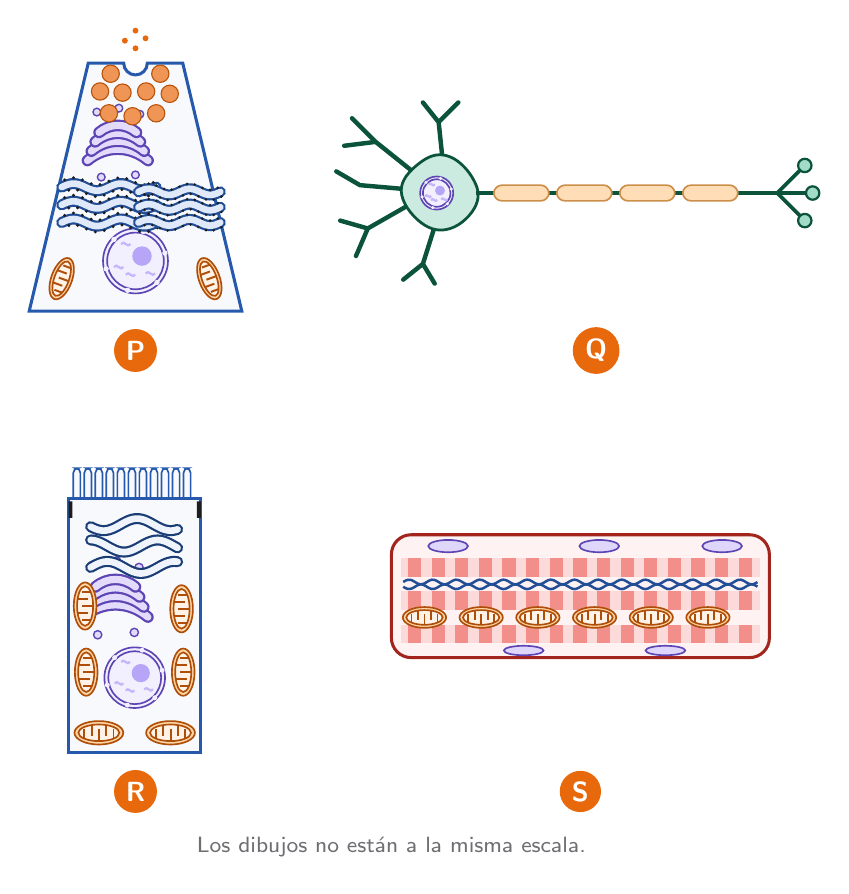
\begin{tikzpicture}[font=\small]

\begin{scope}[scale=0.75]
\draw[azul!80!black,fill=azul!4,line width=1.1pt] (0,0) -- (3.6,0) -- (2.6,4.2) -- (2.0,4.2) arc[start angle=0,end angle=-180,radius=0.2] -- (1.0,4.2) -- cycle;
\foreach \p in {(1.8,4.45),(1.62,4.58),(1.97,4.62),(1.8,4.75)} \fill[nar] \p circle (0.05);
\nucleo{1.8}{0.85}{0.55}
\pic at (0.55,1.5) [scale=0.75] {rer};
\pic at (1.85,1.5) [scale=0.65] {rer};
\pic at (1.5,2.55) [rotate=90,scale=0.7] {golgi};
\foreach \p in {(1.35,3.35),(1.75,3.3),(2.15,3.35),(1.2,3.72),(1.58,3.7),(1.98,3.72),(2.38,3.68),(1.38,4.02),(2.22,4.02)} \pic at \p {gran};
\pic at (0.55,0.55) [rotate=70,scale=0.55] {mito};
\pic at (3.05,0.55) [rotate=110,scale=0.55] {mito};
\end{scope}
\node[circle,fill=nar,text=white,font=\bfseries,inner sep=2pt] at (1.35,-0.5) {P};
\begin{scope}[xshift=5.2cm,yshift=1.5cm,scale=0.5]
\draw[menta!50!black,line width=1.6pt,line cap=round] (-0.6,0.5) -- (-1.6,1.3) -- (-2.2,1.9) (-1.6,1.3) -- (-2.4,1.2) (-0.75,-0.3) -- (-1.8,-0.9) -- (-2.5,-0.7) (-1.8,-0.9) -- (-2.1,-1.6) (0.1,0.85) -- (0.0,1.8) -- (-0.4,2.3) (0.0,1.8) -- (0.5,2.3) (-0.1,-0.85) -- (-0.4,-1.8) -- (-0.1,-2.3) (-0.4,-1.8) -- (-0.9,-2.2) (-0.85,0.1) -- (-2.0,0.2) -- (-2.6,0.55);
\draw[menta!50!black,fill=menta!22,line width=1pt] plot[smooth cycle,tension=0.7] coordinates {(-0.95,0.05)(-0.5,0.75)(0.2,0.95)(0.85,0.4)(0.95,-0.3)(0.3,-0.9)(-0.45,-0.75)};
\nucleo{-0.05}{0.0}{0.42}
\draw[menta!50!black,line width=1.6pt] (0.95,0) -- (8.6,0);
\foreach \x in {1.4,3.0,4.6,6.2} \draw[narc!80!black,fill=narc!45,line width=0.6pt,rounded corners=3pt] (\x,-0.2) rectangle (\x+1.4,0.2);
\draw[menta!50!black,line width=1.3pt,line cap=round] (8.6,0) -- (9.3,0.7) (8.6,0) -- (9.5,0) (8.6,0) -- (9.3,-0.7);
\foreach \p in {(9.3,0.7),(9.5,0),(9.3,-0.7)} \draw[menta!50!black,fill=menta!40,line width=0.8pt] \p circle (0.17);
\end{scope}
\node[circle,fill=nar,text=white,font=\bfseries,inner sep=2pt] at (7.2,-0.5) {Q};
\begin{scope}[xshift=0.5cm,yshift=-5.6cm,scale=0.7]
\foreach \x in {0.15,0.35,...,2.3} \draw[azul!80!black,fill=azul!4,line width=0.6pt,rounded corners=0.06cm] (\x-0.065,4.4) rectangle (\x+0.065,5.15);
\draw[azul!80!black,fill=azul!4,line width=1.1pt] (0,0) rectangle (2.4,4.6);
\fill[tinta] (0,4.25) rectangle (0.07,4.55) (2.33,4.25) rectangle (2.4,4.55);
\nucleo{1.2}{1.35}{0.55}
\pic at (0.85,2.45) [rotate=90,scale=0.75] {golgi};
\pic at (0.4,3.35) [scale=0.85] {rel};
\pic at (0.55,0.35) [scale=0.62] {mito};
\pic at (1.85,0.35) [scale=0.62] {mito};
\pic at (0.32,1.45) [rotate=90,scale=0.6] {mito};
\pic at (2.08,1.45) [rotate=90,scale=0.6] {mito};
\pic at (2.05,2.6) [rotate=90,scale=0.6] {mito};
\pic at (0.3,2.65) [rotate=90,scale=0.6] {mito};
\end{scope}
\node[circle,fill=nar,text=white,font=\bfseries,inner sep=2pt] at (1.35,-6.1) {R};
\begin{scope}[xshift=4.6cm,yshift=-4.4cm,scale=0.6]
\draw[coral!70!black,fill=coral!6,line width=1.1pt,rounded corners=0.25cm] (0,0) rectangle (8,2.6);
\foreach \ya/\yb in {0.3/0.7,1.0/1.4,1.7/2.1} {
  \fill[coral!18] (0.2,\ya) rectangle (7.8,\yb);
  \foreach \x in {0.35,0.85,...,7.4} \fill[coral!55] (\x,\ya) rectangle (\x+0.28,\yb);
}
\foreach \x in {0.7,1.9,3.1,4.3,5.5,6.7} \pic at (\x,0.85) [scale=0.55] {mito};
\draw[azul!70!black,line width=0.9pt] plot[domain=0.25:7.75,samples=150,smooth] (\x,{1.5+0.05*sin(\x*720)});
\draw[azul!70!black,line width=0.9pt] plot[domain=0.25:7.75,samples=150,smooth] (\x,{1.6-0.05*sin(\x*720)});
\foreach \x in {1.2,4.4,7.0} \draw[lila!75!black,fill=lila!25,line width=0.6pt] (\x,2.36) ellipse (0.42 and 0.13);
\foreach \x in {2.8,5.8} \draw[lila!75!black,fill=lila!25,line width=0.6pt] (\x,0.15) ellipse (0.42 and 0.1);
\end{scope}
\node[circle,fill=nar,text=white,font=\bfseries,inner sep=2pt] at (7.0,-6.1) {S};
\node[font=\footnotesize,text=gris] at (4.6,-6.8) {Los dibujos no están a la misma escala.};

\end{tikzpicture}
\end{document}
